\label{sec:dthreads-architecture}

This section describes \dthreads{}' key algorithms---mem\-ory
isolation, deterministic (diff-based) memory commit, deterministic
synchronization, and deterministic memory allocation---as well as
other implementation details.

\subsection{Isolated Memory Access}

\label{sec:threadsasprocs}
To achieve deterministic memory access, 
\dthreads{} isolates memory accesses among different
threads between commit points, and commits the updates of each thread deterministically.

\dthreads{} achieves cross-thread memory isolation by 
replacing threads with processes.  In a multithreaded program running
with \pthreads{}, threads share all memory except for the stack.  Changes
to memory immediately become visible to all other threads.  Threads share
the same file descriptors, sockets, device handles, and windows.
By contrast, because \dthreads{} runs threads in separate processes, it must manage these shared
resources explicitly.

\begin{figure}[h]
{\centering
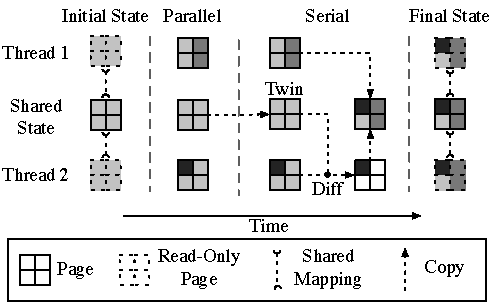
\includegraphics{fig/architecture-diagram}
\caption{An overview of \dthreads{} execution.\label{fig:architecture}}
}
\end{figure}

\subsubsection{Thread Creation}

\dthreads{} replaces the \texttt{pthread\_create()} function with
the \texttt{clone} system call provided by Linux. To create
processes that have disjoint address spaces but share the same file descriptor table, \dthreads{} uses the \texttt{CLONE\_FILES} flag.
\dthreads{} shims the \texttt{getpid()} function to return a single, globally-shared identifier.

\subsubsection{Deterministic Thread Index}
\label{sec:threadindex}
POSIX does not guarantee deterministic process or thread identifiers;
that is, the value of a process id or thread id is not deterministic.
To avoid exposing this non-determinism to threads running as
processes, \dthreads{} shims
\texttt{pthread\_self()} to return an internal thread index.
The internal thread index is managed using a single global variable
that is incremented on thread creation.  This unique thread index is
also used to manage per-thread heaps and as an offset into an array of
thread entries.

%\subsubsection{Stack and Heap} 
% TTT: Change the title since we don't care about stack and add the mapping information, otherwise, it is not clear how we
% do that, it is very important to do so.
\subsubsection{Shared Memory}
\label{sec:stackandheap}

To create the illusion of different threads sharing the same
address space, \dthreads{} uses memory mapped files to share memory
across processes (globals and the heap, but not the stack; see
Section~\ref{sec:discussion}).

\dthreads{} creates two different mappings for both the heap and the
globals.  One is a \emph{shared} mapping, which is used to hold shared state.
The other is a \emph{private}, copy-on-write (COW) per-process mapping that
each process works on directly.  Private mappings are linked to the
shared mapping through a single fixed-size memory-mapped file.
Reads initially go directly to the shared mapping,
but after the first write operation,
both reads and writes are entirely private.

Memory allocations from the shared heap use a scalable
per-thread heap organization loosely based on
Hoard~\cite{BergerMcKinleyBlumofeWilson:ASPLOS2000} and built using
HeapLayers~\cite{BergerZornMcKinley:2001}.  \dthreads{} divides the
heap into a fixed number of sub-heaps (currently 16).  Each thread
uses a hash of its deterministic thread index to find the appropriate sub-heap.

\subsection{Deterministic Memory Commit}
\label{sec:sharedmem}

\begin{figure}[b]
{\centering 
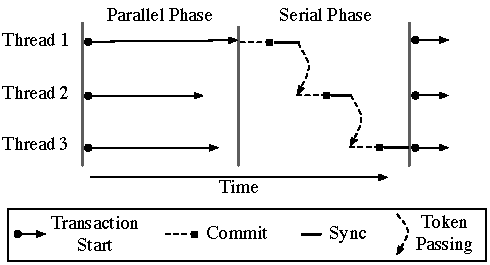
\includegraphics{fig/phase-diagram}
\caption{An overview of \dthreads{} phases. Program execution with \dthreads{} alternates between parallel and serial phases.\label{fig:phase}}
}
\end{figure}

Figure~\ref{fig:phase} illustrates the progression of parallel and serial phases. 
To guarantee determinism, \dthreads{} isolates memory accesses in the parallel phase. These accesses work on private copies of memory; that is, updates are not shared between threads during the parallel phase.
When a synchronization point is reached, updates are applied (and made visible) in a deterministic order.  
This section describes the mechanism used to alternate between parallel and serial execution phases 
and guarantee deterministic commit order, and the details of commits to shared memory.

\subsubsection{Fence and Token}
\label{sec:schedule}

The boundary between the parallel and serial phases is the internal
fence. We implement this fence with a custom barrier, because the
standard \pthreads{} barrier does not support a dynamic thread count
(see Section~\ref{sec:synchronization}).

\punt{
\label{sec:token}
\begin{figure}[ht]
\begin{lstlisting}
void waitFence(void) {
	lock();
	while(!isArrivalPhase()) { 
		CondWait();
	}

	waiting_threads++;
	if(waiting_threads < live_threads) {
		while(!isDeparturePhase()) {
			CondWait();
		}
	} else {
		setDeparturePhase();
		CondBroadcast();
	}

	waiting_threads--;
	if (waiting_threads == 0) {
		setArrivalPhase();
		CondBroadcast();
	}
	unlock();
}
\end{lstlisting}
\caption{Pseudocode for \dthreads{}' internal fence. ($\S$ \ref{sec:schedule})
\label{fig:internalFence}}
\end{figure}
}

\punt{
Figure~\ref{fig:internalFence} presents pseudocode for the internal fence.
Threads must wait at the fence 
until all threads from the previous 
If the thread is the last to enter the fence, it sets the departure phase and wakes the waiting threads (lines 12-15).  
As threads leave the fence, they decrement the waiting thread count.  The last thread to leave sets the fence to the arrival phase and wakes any waiting threads (lines 17-21).
}

Threads wait at the internal fence until all threads from the
previous fence have departed. Waiting threads must block until
the departure phase. If the thread is the last to enter the fence, it
initiates the departure phase and wakes all waiting threads.  As threads
leave the fence, they decrement the waiting thread count.  The last
thread to leave sets the fence to the arrival phase and wakes any
waiting threads.

To reduce overhead, whenever the number of running threads is less than or equal
to the number of cores, waiting threads block by spinning rather
than by invoking relatively expensive cross-process \pthreads{}
mutexes. When the number of threads exceeds the number of
cores, \dthreads{} falls back to using \pthreads{} mutexes.

\punt{
\begin{figure}[!t]
\begin{lstlisting}
void waitToken() {
	waitFence();
	while(token_holder != thread_id) {
		yield();
	}
}
void putToken() {
	token_holder = token_queue.nextThread();
}
\end{lstlisting}
\caption{Pseudocode for token management ($\S$ \ref{sec:schedule}).
\label{fig:token}}
\end{figure}
}

A key mechanism used by \dthreads{} is its global token.
To guarantee determinism, each thread must wait for the token
before it can communicate with other threads. 
The token is a shared pointer that points to the next runnable thread entry.
Since the token is unique in the entire system, waiting for the token guarantees a global order for
all operations in the serial phase. 

\dthreads{} uses two internal subroutines to manage tokens. The \texttt{waitToken} function
first waits at the internal fence and then waits to acquire the global token
before entering serial mode. The \texttt{putToken} function passes the token to
the next waiting thread.

To guarantee determinism (see Figure~\ref{fig:phase}), threads leaving the parallel phase 
must wait at the internal fence before they can enter into the serial phase (by calling
\texttt{waitToken}).
Note that it is crucial that threads wait at the fence even for a thread which is guaranteed to obtain the token next,
since one thread's commits can affect another threads' behavior if there is no fence.

% XXX EDB FIX ME -- commented out because I do not get this.

%In the serial phase, each thread can perform those commits for parallel phase and actual synchronizations
%before they passed the token to next thread. 
%At the end of serial phase, each thread must wait at the fence before resuming execution.


%\textbf{CCC: Edited}

\subsubsection{Commit Protocol}
\label{sec:protocol}

Figure~\ref{fig:architecture} shows the steps taken by \dthreads{} to
capture modifications to shared state and expose them in a
deterministic order.  At the beginning of the parallel phase, threads
have a read-only mapping for all shared pages.  If a thread writes to
a shared page during the parallel phase, this write is trapped and
re-issued on a private copy of the shared page.  Reads go directly to
shared memory and are not trapped.  In the serial phase, threads
commit their updates one at a time.  The first thread to commit to a
page can directly copy its private copy to the shared state, but
subsequent commits must copy only the modified bytes.  \dthreads{} 
computes diffs from a twin page, an unmodified copy of the shared page created at 
the beginning of the serial phase.  At the end of the serial phase,
private copies are released and these addresses are restored to
read-only mappings of the shared memory.

\punt{
\begin{figure}[!t]
\begin{lstlisting}
void atomicBegin() {
	foreach(page in modifiedPages) {
		page.writeProtect();
		page.privateCopy.free();
	}
	modifiedPages.emptyList()
}
\end{lstlisting}
\caption{Pseudocode for \texttt{atomicBegin} ($\S$ \ref{sec:atomicbegin}).\label{fig:atomicbegin}}
\end{figure}
}

\punt{
Figure~\ref{fig:atomicbegin} presents pseudocode for
\texttt{atomicBegin}.  First, all previously-written
pages are write-protected (line 3).  The old working copies of these
pages are then discarded, and mappings are updated to reference the
shared state (line 4).
}

\label{sec:atomicbegin}

At the start of every transaction (that is, right after a
synchronization point), \dthreads{} starts by write-protecting all
previously-written pages. The old working copies of these pages are
then discarded, and mappings are then updated to reference the shared
state.

\punt{
\begin{figure}[!t]
\begin{lstlisting}
void atomicEnd() {
	foreach(page in modifiedPages) {
		if(page.writers > 1 && !page.hasTwin()) {
			page.createTwin();
		}
		if(page.version == page.localCopy.version) {
			page.copyCommit();
		} else {
			page.diffCommit();
		}
		page.writers--;
		if(page.writers == 0 && page.hasTwin()) { 
			page.twin.free();
		}
		page.version++;
	}
}
\end{lstlisting}
\caption{Pseudocode for \texttt{atomicEnd} ($\S$ \ref{sec:atomicbegin}).
\label{fig:atomicend}}
\end{figure}
}

\punt{
Figure~\ref{fig:atomicend} presents pseudocode for
\texttt{atomicEnd}.  \texttt{atomicEnd} commits all
changes from the current transaction to the shared page.  For each
modified page with more than one writer, \dthreads{} ensures that a
twin page is created (lines 3-5).  If the version number of the
private copy matches the shared page, then the current thread must be the first thread to
commit.  In this case, the entire private copy can be copied to the
shared state (lines 7 and 8).  If the version numbers do not match,
then another thread has already committed changes to the page and a
diff-based commit must be used (lines 9-10).
After changes have been committed, the number of writers to the
page is decremented (line 13), and if there are no writers left to
commit, the twin page is freed (lines 14-16).  Finally, the shared
page's version number is incremented (line 17).
}

Just before every synchronization point, \dthreads{} first waits for
the global token (see below), and then commits all changes from the
current transaction to the shared pages in order. \dthreads{} maintains one
``twin'' page (a snapshot of the original) for every modified page
with more than one writer. If the version number of the private copy
matches the shared page, then the current thread must be the first
thread to commit.  In this case, the working copy can be copied directly
to the shared state.  If the version numbers do not match, then
another thread has already committed changes to the page and a
diff-based commit must be used.

Once changes have been committed, the number of writers to the
page is decremented and the shared page's version number is incremented.
If there are no writers left to commit, the twin page is freed.

\subsection{Deterministic Synchronization}
\label{sec:synchronization}

%Comparing to Grace, \dthreads{} supports one complete synchronization
%mechanism.  Grace turns lock operations to no-ops to eliminate
%deadlocks and does not support condition variables or barriers.  The
%only supported synchronization by Grace is thread exit; Grace enforces
%a sequential semantics in thread exit.
%
\dthreads{} enforces determinism for the full range of synchronization operations in the
\pthreads{} API, including locks, condition variables, barriers and
various flavors of thread exit.

\subsubsection{Locks}
\label{sec:lock}

\dthreads{} uses a single global token to guarantee ordering and atomicity during the serial phase.  When acquiring a lock, threads must first wait for the global token.  Once a thread has the token it can attempt to acquire the lock.  If the lock is currently held, the thread must pass the token and wait until the next serial phase to acquire the lock.  It is possible for a program run with \dthreads{} to deadlock, but only for programs that can also deadlock with \pthreads{}.

% EDB: We need to acquire a token before we can execute any
% synchronization operation. We only release the token once our lock
% count is 0 (for instance, lock(A); lock(B); unlock(B); unlock(A);
% we release the token only after unlock(A).

\punt{
\begin{figure}[ht]
\begin{lstlisting}
void mutex_lock() { if(lock_count == 0) { waitToken(); atomicEnd();
	atomicBegin(); } lock_count++; }
\end{lstlisting}
\caption{Pseudocode for \texttt{mutex\_lock} ($\S$ \ref{sec:lock}).
\label{fig:lock}}
\end{figure}
}

\punt{
Figure~\ref{fig:lock} presents the pseudocode for lock acquisition.  First, \dthreads{} checks to see if the current thread is already holding any locks.  If not, the thread first waits for the token, commits changes to shared state by calling \texttt{atomicEnd}, and begins a new atomic section (lines 2-6).  Finally, the thread increments the number of locks it is currently holding.  This count must be kept to ensure that a thread will not pass the token until it has release all of the locks it acquired in the serial phase.
}

Lock acquisition proceeds as follows. First, \dthreads{} checks 
to see if the current thread is already holding any locks.  If not, the thread first waits for the token, commits changes to shared state by calling \texttt{atomicEnd}, and begins a new atomic section.  Finally, the thread increments the number of locks it is currently holding.  The lock count ensures that a thread does not pass the token on until it has released all of the locks it acquired in the serial phase.

\punt{
\begin{figure}[ht]
\begin{lstlisting}
void mutex_unlock(){
	lock_count--;
	if(lock_count == 0) {
		atomicEnd();
		putToken();
		atomicBegin();
		waitFence();
	}
}
\end{lstlisting}
\caption{Pseudocode for \texttt{mutex\_unlock} ($\S$ \ref{sec:lock}).
\label{fig:unlock}}
\end{figure}
}

\punt{
Figure~\ref{fig:unlock} presents the implementation of \texttt{pthread\_mutex\_unlock}.  First, the thread decrements its lock count (line 2).  If no more locks are held, any local modifications are committed to shared state, the token is passed, and a new atomic section is started (lines 3-6).  Finally, the thread waits on the internal fence until the start of the next round's parallel phase (line 7).
}

\texttt{pthread\_mutex\_unlock}'s implementation is similar.  First,
the thread decrements its lock count.  If no more locks are held, any
local modifications are committed to shared state, the token is
passed, and a new atomic section is started.  Finally, the thread
waits on the internal fence until the start of the next round's
parallel phase. If other locks are still held, the lock count is just
decreased and the running thread continues execution with the global
token.


\subsubsection{Condition Variables}
\label{sec:condwait}

Guaranteeing determinism for condition variables is more complex than for mutexes because the operating system does not guarantee that processes will wake up in the order they waited for a condition variable.

\punt{
\begin{figure}[ht]
\begin{lstlisting}
void cond_wait() {
	waitToken();
	atomicEnd();
	
	token_queue.removeThread(thread_id);
	live_threads--;
	cond_queue.addThread(thread_id);
	putToken();	

	while(!threadReady()) {
		real_cond_wait();
	}
	
	while(token_holder != thread_id) {
		yield();
	}
	atomicBegin();
}
\end{lstlisting}
\caption{Pseudocode for \texttt{pthread\_cond\_wait} ($\S$~\ref{sec:condwait}). 
\label{fig:condwait}}
\end{figure}
}

\punt{
Figure~\ref{fig:condwait} presents pseudocode for the \dthreads{} implementation of \texttt{pthread\_cond\_wait}.  When a thread calls \texttt{pthread\_cond\_wait}, it first waits for the token and commits local modifications (lines 2 and 3).  It removes itself from the token queue (line 4) because threads waiting on a condition variable do not participate in the serial phase until they are woken up.  The thread decrements the live thread count (used for the fence between parallel and serial phases), adds itself to the condition variable's queue, and passes the token (lines 6-8).  While threads are waiting on \dthreads{} condition variables, they are suspended on a \pthreads{} condition variable (lines 10-12).  Once a thread is woken up, it busy-waits on the token and finally begins the next transaction (lines 14-17).  Threads must acquire the token (to ensure serial execution) before proceeding because \texttt{pthread\_cond\_wait} is called within a mutex's critical section.
}

When a thread calls \texttt{pthread\_cond\_wait}, it first acquires
the token and commits local modifications.  It then removes itself
from the token queue, because threads waiting on a condition variable
do not participate in the serial phase until they are awakened.  The
thread decrements the live thread count (used for the fence between
parallel and serial phases), adds itself to the condition variable's
queue, and passes the token.  While threads are waiting on \dthreads{}
condition variables, they are suspended on a \pthreads{} condition
variable.  When a thread is awakened (signalled), it busy-waits on the
token before beginning the next transaction.  Threads must
acquire the token before proceeding
because the condition variable wait function must be called within a mutex's
critical section.

\label{sec:condsignal}

\punt{
\begin{figure}[ht]
\begin{lstlisting}
void cond_signal() {
	if(token_holder != thread_id) {
		waitToken();
	}
	atomicEnd();
	
	if(cond_queue.length == 0) {
		return;
	}
	
	lock();
	thread = cond_queue.removeNext();
	token_queue.insert(thread);
	live_threads++;
	thread.setReady(true);
	real_cond_signal();
	unlock();
	atomicBegin();
}
\end{lstlisting}
\caption{Pseudocode for \texttt{pthread\_cond\_signal} ($\S$~\ref{sec:condsignal}). 
\label{fig:condsignal}}
\end{figure}
}

\punt{
The \dthreads{} implementation of \texttt{pthread\_cond\_signal} is presented in Figure~\ref{fig:condsignal}.  The calling thread first waits for the token, and then commits any local modifications (lines 2-5).  If no threads are waiting on the condition variable, this function returns immediately (lines 7-9).  Otherwise, the first thread in the condition variable queue is moved to the head of the token queue and the live thread count is incremented (lines 12-14).  This thread is then marked as ready and woken up from the real condition variable, and the calling thread begins another transaction (lines 15-18).
}

In the \dthreads{} implementation of \texttt{pthread\_cond\_signal},
the calling thread first waits for the token, and then commits any
local modifications.  If no threads are waiting on the condition
variable, this function returns immediately.  Otherwise, the first
thread in the condition variable queue is moved to the head of the
token queue and the live thread count is incremented.  This thread is
then marked as ready and woken up from the real condition variable,
and the calling thread begins another transaction.

To impose an order on signal wakeup, \dthreads{} signals
actually call 
\texttt{pthread\_cond\_broadcast} to wake all waiting threads, but then marks only
the logically next one as ready.  The threads not marked as
ready will wait on the condition variable again.

\subsubsection{Barriers}

\label{sec:barrierwait}

As with condition variables, \dthreads{} must ensure that threads
waiting on a barrier do not disrupt token passing among running
threads. \dthreads{} removes threads entering into the barrier from
the token queue and places them on the corresponding barrier queue.

In \texttt{pthread\_barrier\_wait}, the calling thread first waits for
the token to commit any local modifications. If the current thread is
the last to enter the barrier, then \dthreads{} moves the entire list
of threads on the barrier queue to the token queue, increases the
live thread count, and passes the token to the first thread in the
barrier queue.  Otherwise, \dthreads{} removes the current thread from
the token queue, places it on the barrier queue, and releases
token. Finally, the thread waits on the actual \pthreads{} barrier.

\punt{
\begin{figure}[ht]
\begin{lstlisting}
void barrier_wait() {
	waitToken();
	atomicEnd();
	lock();
	if(barrier_queue.length == barrier_count-1) {
		token_holder = barrier_queue.first();
		live_threads += barrier_queue.length;
		barrier_queue.moveAllTo(token_queue);
	} else {
		token_queue.remove(thread_id);
		barrier_queue.insert(thread_id);
		putToken();
	}
	unlock();
	atomicBegin();
	real_barrier_wait();
}
\end{lstlisting}
\caption{Pseudocode for barrier\_wait ($\S$~\ref{sec:barrierwait}).
\label{fig:barrierwait}}
\end{figure}
}

\punt{
Figure~\ref{fig:barrierwait} presents pseudocode
for \texttt{pthread\_barrier\_wait}. The calling thread first waits for the
token to commit any local modifications in order to ensure
deterministic commit (lines 2 and 3). If the current thread is the
last to enter the barrier, then \dthreads{} moves the entire list of
threads on the barrier queue to the token queue (line 7), increases
the fence's thread count (line 8), and passes the token to the first thread in the
barrier queue (line 9).  Otherwise, \dthreads{} removes the current
thread from the token queue (line 12), places it on the barrier queue
(line 13), and releases token (line 14). Finally, the thread waits on
the actual barrier (line 19).
}

\subsubsection{Thread Creation and Exit}

\label{sec:threadcreation}

To guarantee determinism, thread creation and exit are performed
in the serial phase.  Newly-created threads are added to
the token queue immediately after the parent thread.  Creating a thread does not  release the token; this approach allows a single thread to quickly create multiple child threads without having to wait for a new serial phase for each child thread.

\punt{
\begin{figure}[ht]
\begin{lstlisting}
void thread_create() {
	waitToken();
	clone(CLONE_FS | CLONE_FILES | CLONE_CHILD);
	if(child_process) {
		thread_id = next_thread_index;
		next_thread_index++;
		notifyChildRegistered();
		waitParentProadcast();
	} else {
		waitChildRegistered();
	}
}
\end{lstlisting}
\caption{Pseudocode for \texttt{thread\_create} ($\S$ \ref{sec:threadcreation}).
\label{fig:threadcreate}}
\end{figure}
}

\punt{
Figure~\ref{fig:threadcreate} presents pseudocode for thread
creation. The caller first waits for the token before proceeding (line
2).  It then creates a new process with shared file descriptors but a
distinct address space using the \texttt{clone} system call (line 3).
The newly created child obtains the global thread index (line 5),
places itself in the token queue (line 6), and notifies the parent
that child has registered itself in the active list (line 7). The
child thread then waits for the parent to reach a synchronization
point.
}

When creating a thread, the parent first waits for the token. It then
creates a new process with shared file descriptors but a distinct
address space using the \texttt{clone} system call.  The newly created
child obtains the global thread index, places itself in the token
queue, and notifies the parent that the child has registered itself in the
active list. The child thread then waits for the next parallel phase before proceeding.

\punt{
\begin{figure}[ht]
\begin{lstlisting}
void thread_exit() {
	waitToken();
	atomicEnd();
	token_queue.remove(thread_id);
	live_threads--;
	putToken();
	real_thread_exit();
}
\end{lstlisting}
\caption{Pseudocode for \texttt{thread\_exit} ($\S$ \ref{sec:threadcreation}).
\label{fig:threadexit}}
\end{figure}
}

% \textbf{CCC: Edited}

\punt{
Figure~\ref{fig:threadexit} presents pseudocode for \texttt{thread\_exit}.
When this function is called, the caller first waits for the
token and then commits any local modifications (line 3). It then
removes itself from the token queue (line 4) and decreases the number
of threads required to proceed to the next phase (line 5). Finally,
the thread passes its token to the next thread in the token queue
(line 6) and exits (line 7).
}

Similarly, \dthreads{}' \texttt{pthread\_exit} first waits for the
token and then commits any local modifications to memory. It then
removes itself from the token queue and decreases the number
of threads required to proceed to the next phase. Finally,
the thread passes its token to the next thread in the token queue
 and exits.

%% \vfill %%% EDB

\subsubsection{Thread Cancellation}

\dthreads{} implements thread cancellation in the serial
phase. A thread can only invoke \texttt{pthread\_cancel} while holding the
token.  If the thread being cancelled is waiting on a condition
variable or barrier, it is removed from the queue. Finally, to cancel
the corresponding thread, \dthreads{} kills the target process
with a call to \texttt{kill(tid, SIGKILL)}.


\subsection{Deterministic Memory Allocation}

Programs sometimes rely on the addresses of objects returned by the memory
allocator intentionally (for example, by hashing objects based on
their addresses), or accidentally. A program with a memory error like
a buffer overflow will yield different results for different memory
layouts.

This reliance on memory addresses can undermine other efforts to
provide determinism. For example, CoreDet is unable to fully enforce
determinism because it relies on the Hoard scalable memory
allocator~\cite{BergerMcKinleyBlumofeWilson:ASPLOS2000}. Hoard was not
designed to provide determinism and several of its mechanisms, thread
id based hashing and non-deterministic assignment of memory to
threads, lead to non-deterministic execution in CoreDet for
the \texttt{canneal} benchmark.

To preserve determinism in the face of intentional or inadvertent
reliance on memory addresses, we designed the \dthreads{} memory allocator
to be fully deterministic. \dthreads{} assigns subheaps to each thread
based on its thread index (deterministically assigned; see
Section~\ref{sec:threadindex}). In addition to guaranteeing the same
mapping of threads to subheaps on repeated executions, \dthreads{}
allocates superblocks (large chunks of memory) deterministically by
acquiring a lock (and the global token) on each superblock
allocation. Thus, threads always use the same subheaps, and these
subheaps always contain the same superblocks on each execution. The
remainder of the memory allocator is entirely deterministic. The
superblocks themselves are allocated via \mmap{}: while \dthreads{}
could use a fixed address mapping for the heap, we currently simply disable
ASLR to provide deterministic \mmap{} calls.  If a program does not use the
absolute address of any heap object, \dthreads{} can guarantee determinism even
with ASLR enabled.  Hash functions and lock-free algorithms frequently use
absolute addresses, and any deterministic multithreading system must disable
ASLR to provide deterministic results for these cases.

\subsection{OS Support}

\dthreads{} provides shims for a number of system calls both for
correctness and determinism (although it does not enforce
deterministic arrival of I/O events; see
Section~\ref{sec:discussion}).

System calls that write to or read from buffers on the heap (such
as \texttt{read} and \texttt{write}) will fail if the buffers contain
protected pages. \dthreads{} intercepts these calls and touches each
page passed in as an argument to trigger the copy-on-write operation before issuing the real system
call. \dthreads{} conservatively marks all of these pages as modified
so that any updates made by the system will be committed properly.

\dthreads{} also intercepts other system calls that affect
program execution. For example, when a thread
calls \texttt{sigwait}, \dthreads{} behaves much like it does for
condition variables. It removes the calling thread from the token
queue before issuing the system call, and after being awakened the
thread must re-insert itself into the token queue and wait for the token before proceeding.

